\chapter{Technical background}
\label{cha:technical_background}

In this chapter, a briefly explanation of the used tools is given. Links to the official documentation is provided for further reading. This chapter does not intend to be a full documentation of each component, since their developments is very dynamic.

\section{ROS}
\label{sec:ros}

ROS provides standard \textbf{operating system} services such as hardware abstraction, low-level device control, implementation of commonly-used functionality, message-passing between processes, and package management.

The primary goal of ROS is to support code reuse in robotics research and development. ROS is a \textbf{distributed framework} of processes (aka \textit{Nodes}) that enables executables to be individually designed. These processes can be grouped into \textit{\textbf{Packages}}.

The ROS runtime ``graph'' is a peer-to-peer network of processes that are loosely coupled using the ROS communication infrastructure. ROS also implements several different styles of communication.

Summarizing ROS has two basic ``sides'':
\begin{itemize*}
 \item The operating system side ROS as described above,
 \item and a suite of user contributed packages (organized into sets of nodes) that implement functionalities such as: simultaneous localization and mapping, planning, perception, simulation.
\end{itemize*}

The main goal of this thesis is to be a \textbf{ROS calibration package}, in replacement of the old one \cite{pr2_calibration}. For further learning about ROS, an excellent documentation can be found in: \url{www.ros.org}.

\subsection{Roscpp}
\label{sec:roscpp}

Another primary ROS goal is \textit{``language independence''}: the ROS framework is easy to implement in any modern programming language. It is already implemented in:
\begin{itemize*}
 \item Python (\url{http://www.ros.org/wiki/rospy}) and,
 \item C++ (\url{http://www.ros.org/wiki/roscpp}).
\end{itemize*}

\noindent
Roscpp has been used in this thesis.


\subsection{RViz}
\label{sec:rviz}

It is a 3D visualization tool for ROS. It is used to visualize the \textbf{/tf} (section \ref{sec:tf}) and the \textbf{URDF} robot model (section \ref{sec:urdf}). It is also possible to send messages with basic shapes (cube, sphere, cylinder, arrow) to RViz. This Visual markers has been used in order to visualize the 3D points (see Figure \ref{fig:rviz}). For more information: \url{http://www.ros.org/wiki/rviz}.
\begin{figure}[!htbp]
 \centering
 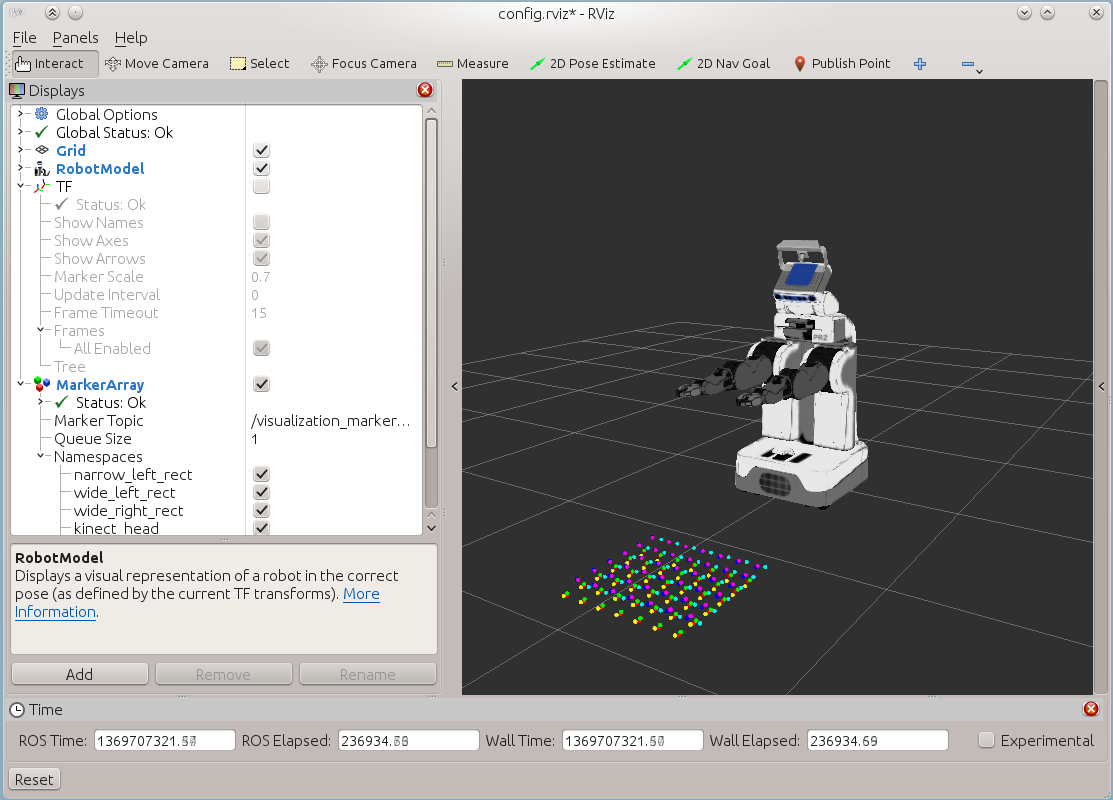
\includegraphics[width=0.95\textwidth]{images/screenshots/rviz.png}
 \caption{RViz interface.}
 \label{fig:rviz}
\end{figure}

\subsection{PR2}
\label{sec:PR2}

The PR2 (Personal Robot, version 2) is a Willow Garage which has two 7-DOF arms with a payload of 1.8 kilograms (1,800 g). Sensors include a 5 megapixel camera, a tilting laser range finder, and an inertial measurement unit. The ``texture projector'' projects a pattern on the environment to create 3D information for capture by the cameras. Also Microsoft Kinect can be head-mounted. In this work, its head (see left on Figure \ref{fig:pr2}) is the most important since all the cameras are located there and most be calibration to each other.
\begin{figure}[!htbp]
 \centering
 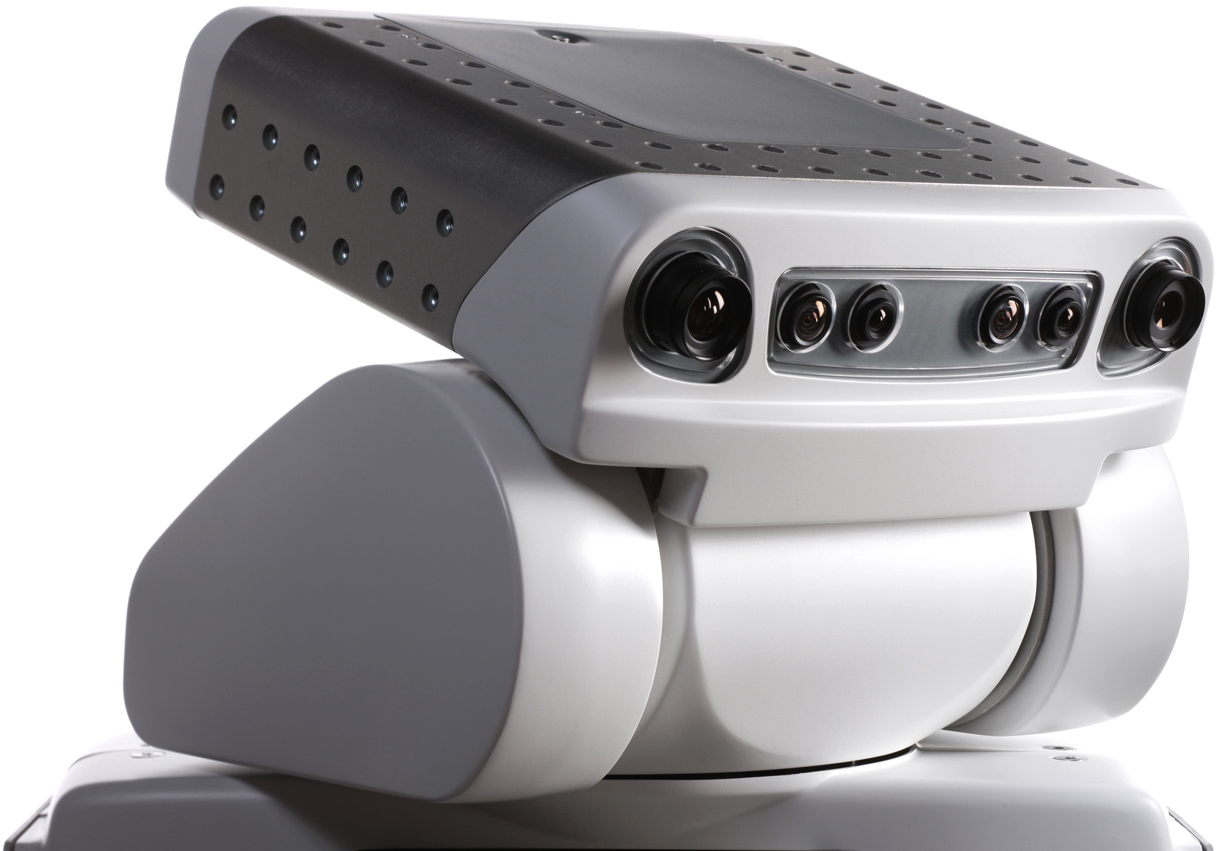
\includegraphics[width=0.45\textwidth]{images/PR2_01.jpg}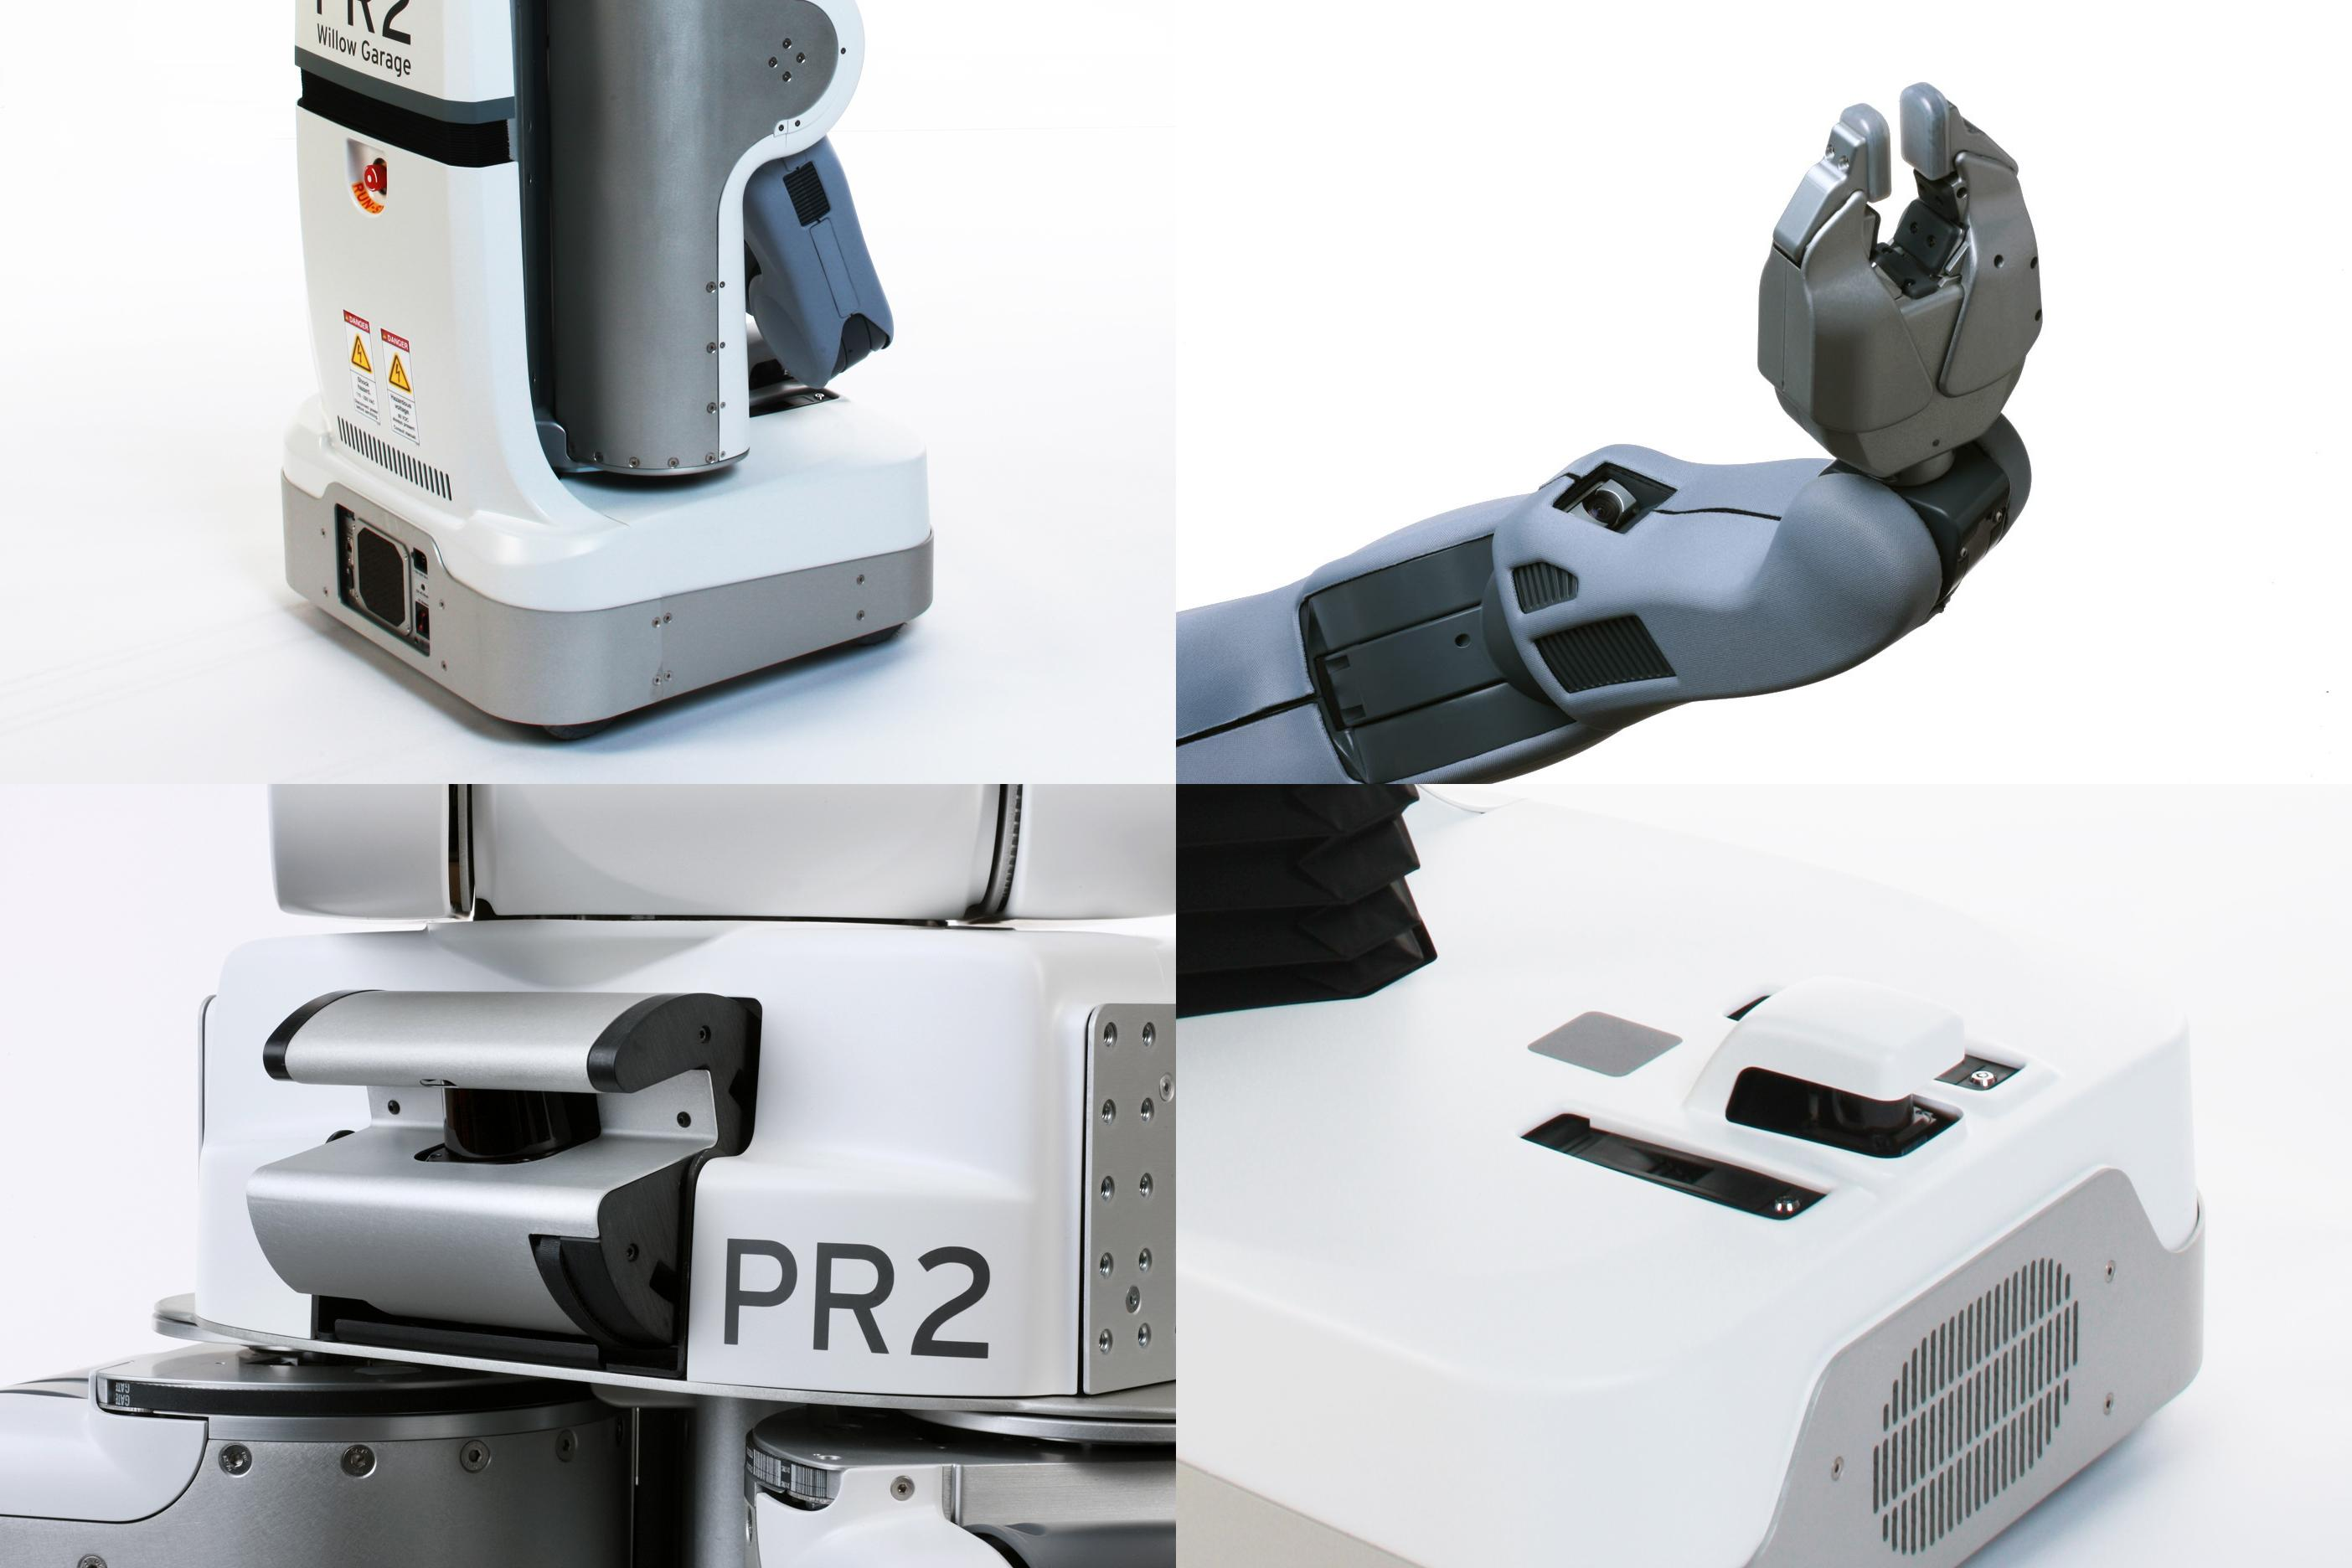
\includegraphics[width=0.45\textwidth]{images/PR2_joint.jpg}
 \caption{PR2 overview}
 \label{fig:pr2}
\end{figure}


\subsection{URDF}
\label{sec:urdf}

The URDF (\textbf{U}nified \textbf{R}obot \textbf{D}escription \textbf{F}ormat) is an XML format for representing a robot model. The package also contains a C++ parser, and it can be visualize with RViz (see in Figure~\ref{fig:pr2_urdf}).
For more information: \url{http://www.ros.org/wiki/urdf}.
\begin{figure}[!htbp]
 \centering
 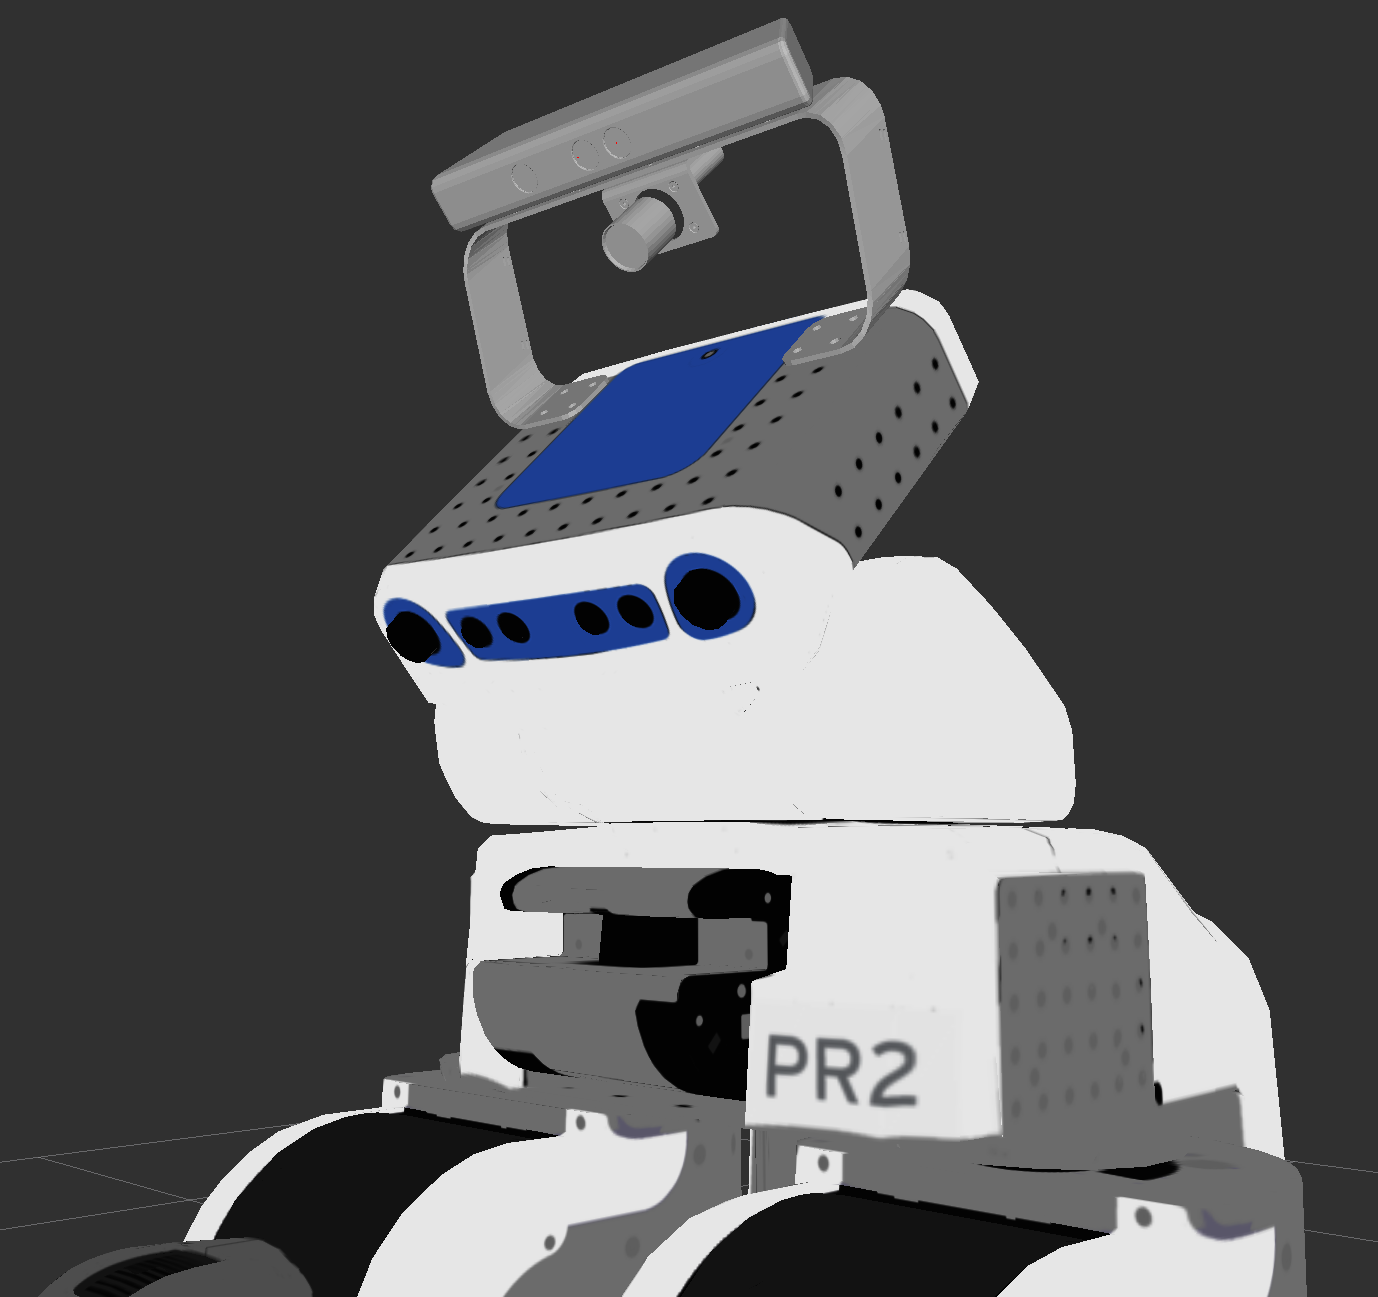
\includegraphics[width=0.35\textwidth]{images/screenshots/PR2_urdf.png}
 \caption{PR2 urdf in RViz}
 \label{fig:pr2_urdf}
\end{figure}


\subsection{/tf}
\label{sec:tf}

The package tf lets the user keep track of multiple coordinate frames over time. tf maintains the relationship between coordinate frames in a tree structure buffered in time, and lets the user transform points, vectors, etc between any two coordinate frames at any desired point in time.

A robotic system typically has many 3D coordinate frames that change over time (see Figure~\ref{fig:tf}), such as a world frame, base frame, gripper frame, head frame, etc. tf keeps track of all these frames over time.
For more information: \url{http://www.ros.org/wiki/tf}.

\begin{figure}[!htbp]
\centering
  \subfigure%[All coordinates system]
  {
    \centering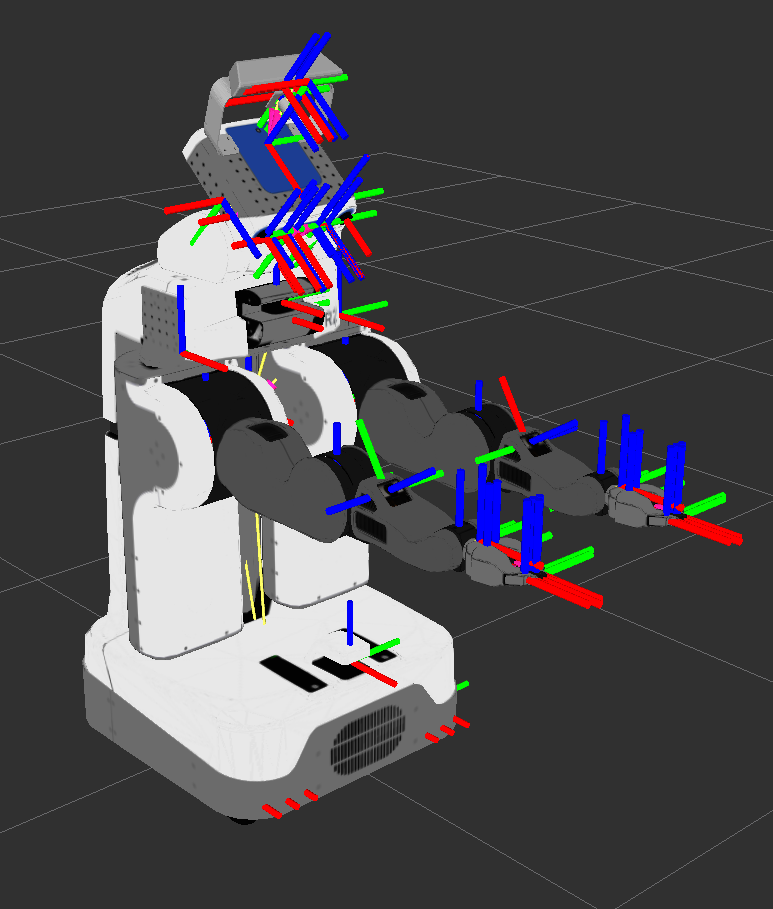
\includegraphics[height=0.3\textheight]{images/screenshots/tf01.png}
    \label{fig:tf01}
  }
  \subfigure%[\texttt{narrow\_stereo\_optical\_frame} until root]
  {
    \centering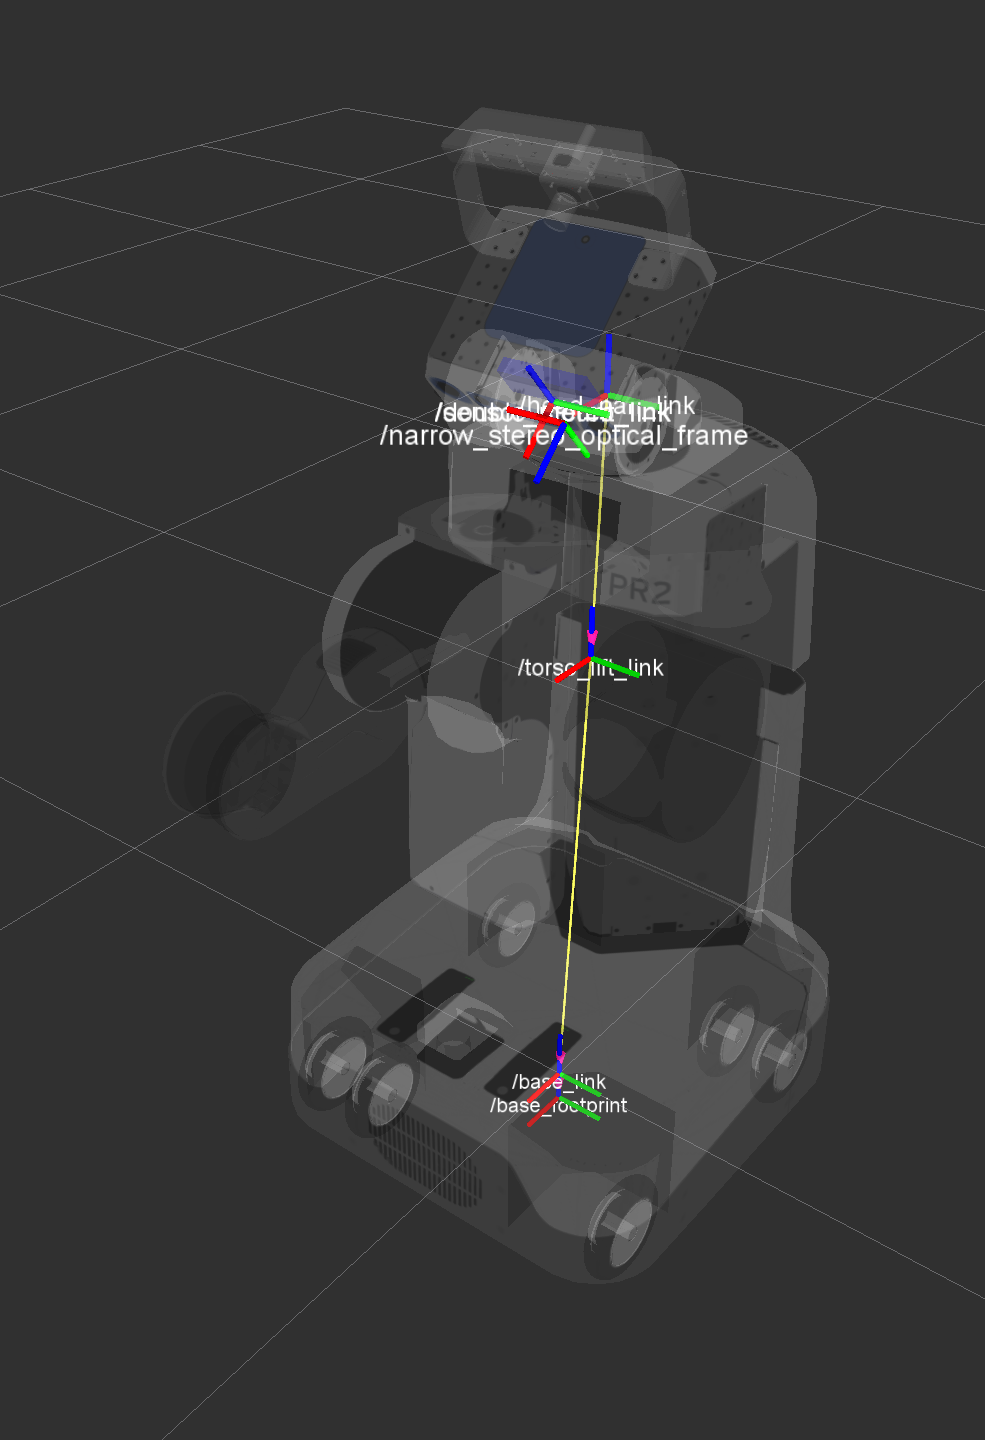
\includegraphics[height=0.3\textheight]{images/screenshots/tf02.png}
    \label{fig:tf02}
  }
  \caption{Example of /tf in RViz (in a particular time). On the left, all coordinates system; on the right, /tf path from \texttt{narrow\_stereo\_optical\_frame} until the robot root (\texttt{base\_footprint}).}
   \label{fig:tf}
\end{figure}


\subsection{ROS bag and rqt}
\label{sec:rosbag}

All the components for a simulated environment are done, and only is needed a way to reproduce events/messages. This is done with ROS bag, which is a set of tools for recording from and playing back to ROS topics. It avoids deserialization and reserialization of the messages. More info: \url{http://www.ros.org/wiki/rosbag}.

\begin{figure}[!htbp]
 \centering
 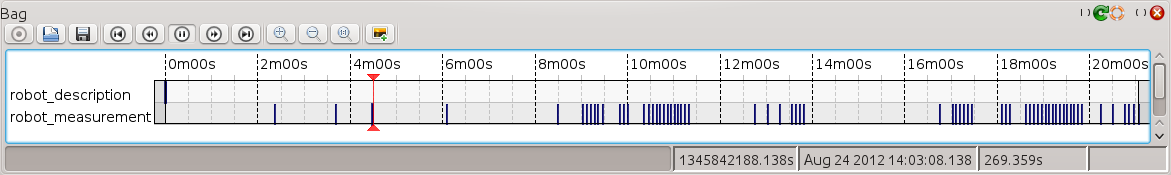
\includegraphics[width=0.95\textwidth]{images/screenshots/rosbag01.png}
 \caption{rqt: \rosbag~interface.}
 \label{fig:rosbag01}
\end{figure}

A second tool described here is a rqt plugin which allows to play a ROS bag easily (Figure~\ref{fig:rosbag01}). The user will be able to see the ROS messages in a convenient way (Figure~\ref{fig:rosbag02}). More info: \url{http://www.ros.org/wiki/rqt}.

\begin{figure}[!htbp]
 \centering
 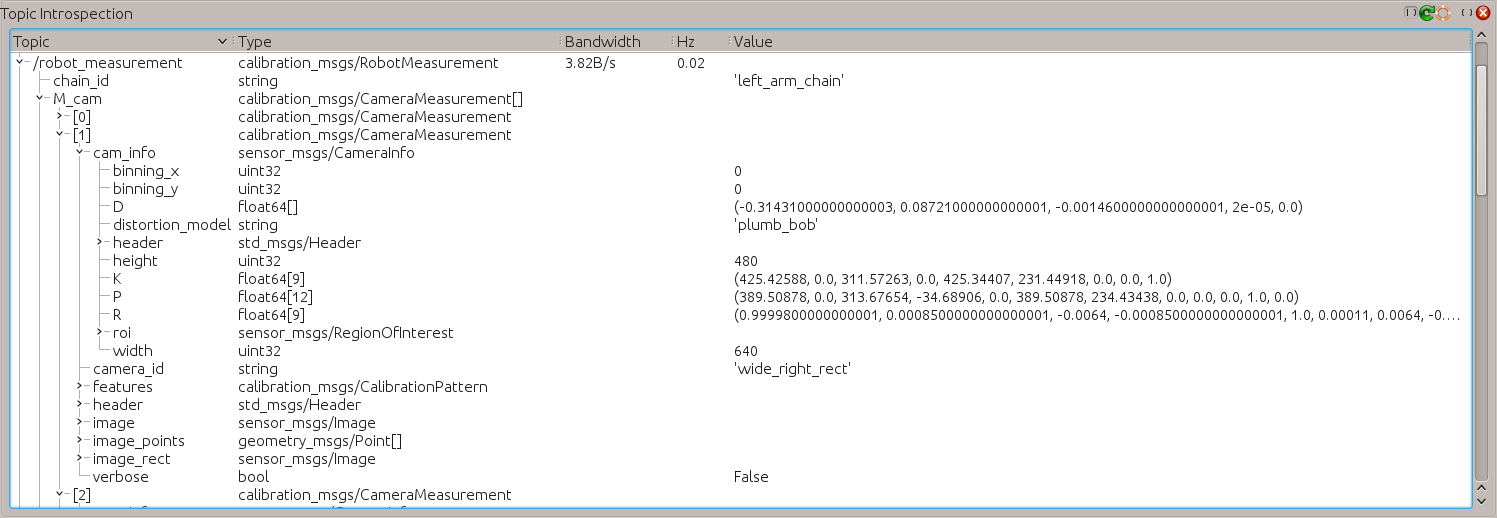
\includegraphics[width=0.95\textwidth]{images/screenshots/rosbag02.png}
 \caption{rqt: Topic introspection.}
 \label{fig:rosbag02}
\end{figure}


\section{KDL}
\label{sec:KDL}

KDL (\textbf{K}inematics and \textbf{D}ynamics \textbf{L}ibrary) defines a tree structure to represent the kinematic and dynamic parameters of a robot mechanism (see Figure \ref{fig:KDL}). \textit{kdl\_parser} provides tools to construct a KDL tree from an XML robot representation in URDf format.

\begin{figure}[!htbp]
 \centering
 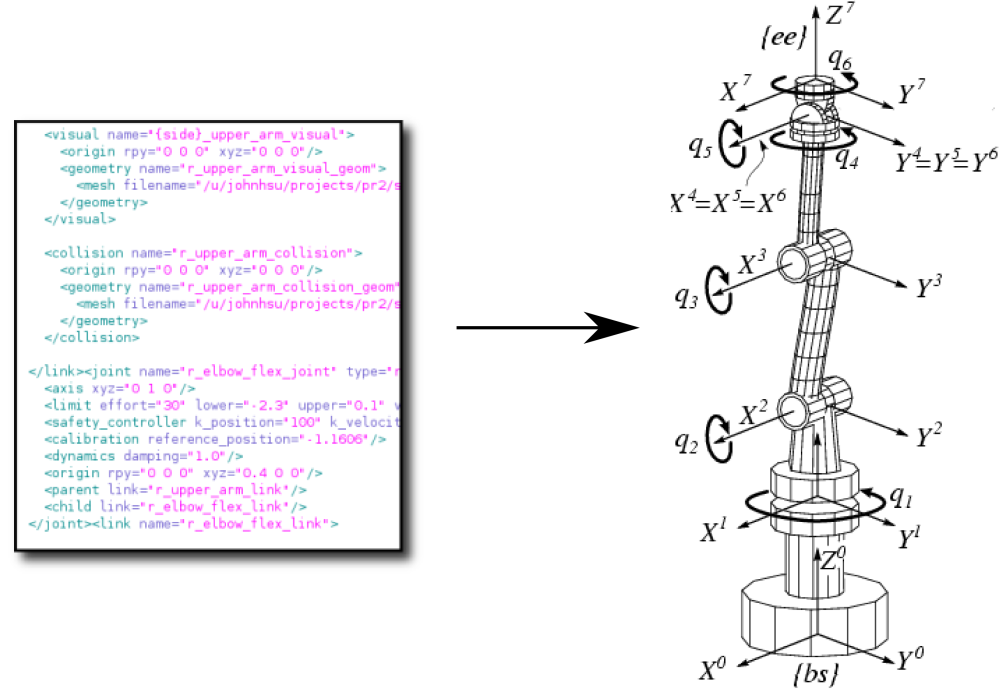
\includegraphics[width=0.7\textwidth]{images/KDL02.png}
 \caption{Example of KDL tree.}
 \label{fig:KDL}
\end{figure}

This library is mainly used for:
\begin{itemize*}
 \item 3D frame and vector transformations,
 \item forward kinematics (given joint angles compute the position of the end-effector\footnote{An \textit{end-effector} is the device at the end of a robotic arm, designed to interact with the environment, in our case the cameras.}).
\end{itemize*}


For more information: \url{http://www.ros.org/wiki/kdl}.

\section{Ceres}
\label{sec:Ceres}

Ceres Solver \cite{ceres} is a portable C++ library that allows modeling and solving large complicated \textbf{non-linear least squares} problems. It is used at Google to estimate the pose of Street View cars, aircrafts, and satellites; to build 3D models for PhotoTours; to estimate satellite image sensor characteristics, and more.

Ceres Solver is an important component in this thesis because, among others, it has very good features like:
\begin{itemize*}
\item A friendly API: build your objective function one term at a time.
\item Automatic Analytic Derivatives.
\item Specialized solvers for bundle adjustment problems in computer vision.
% \item Iterative linear solvers for general sparse and bundle adjustment problems.
\end{itemize*}

It will too long to make a good introduction to Ceres, but a briefly description of important points, obtained from the tutorial, can be found in the following. The excellent tutorial is available in: \url{http://homes.cs.washington.edu/~sagarwal/ceres-solver/tutorial.html}.

\subsection*{Modeling}
Ceres solves robustified non-linear least squares problems of the form:
\[
\frac{1}{2}\sum_{i=1} \rho_i\left(\left\|f_i\left(x_{i_1}, ... ,x_{i_k}\right)\right\|^2\right).
\]

The expression $\rho_i\left(\left\|f_i\left(x_{i_1},...,x_{i_k}\right)\right\|^2\right)$ is known as a \texttt{ResidualBlock}, where $f_i(\cdot)$ is a \texttt{Cost Function} that depends on the parameter blocks $\left[x_{i_1},... , x_{i_k}\right]$. In most optimization problems small groups of scalars occur together. For example, the three components of a translation vector and the four components of the quaternion that define the pose of a camera. We refer to such a group of small scalars as a \texttt{ParameterBlock}. Of course a \texttt{ParameterBlock} can just be a single parameter.

$\rho_i$ is a \texttt{LossFunction}. A \texttt{LossFunction} is a scalar function that is used to reduce the influence of outliers on the solution of non-linear least squares problems. As a special case, when $\rho_i(x) = x$, i.e., the identity function, we get the more familiar non-linear least squares problem.
\[
 \frac{1}{2}\sum_{i=1} \left\|f_i\left(x_{i_1}, ... ,x_{i_k}\right)\right\|^2.
\]

\subsection*{Derivatives}
Ceres Solver like most optimization packages, depends on being able to evaluate the value and the derivatives of each term in the objective function at arbitrary parameter values. Doing so correctly and efficiently is essential to getting good results. Ceres Solver provides a number of ways of doing so: Analytic and Numeric Derivatives. In order to use Automatic differentiation, it is necessary to define a \textbf{templated} cost functor\footnote{A functor is a class with an \texttt{operator()} member. And a cost functor is a functor which evaluate the residuals.}.


